% Demo Presentation - Multi-Agent AI System (Extended with Theory)
\documentclass[aspectratio=169,11pt]{beamer}

% Theme and packages
\usetheme{Madrid}
\usecolortheme{seahorse}
\usepackage{graphicx}
\usepackage{tikz}
\usepackage{listings}
\usepackage{fontawesome5}
\usepackage{array}
\usepackage{booktabs}
\usetikzlibrary{shapes,arrows,positioning,fit,backgrounds}

% Code listing settings
\lstset{
    basicstyle=\ttfamily\tiny,
    keywordstyle=\color{blue},
    breaklines=true,
    frame=single
}

% Title slide information
\title{\textbf{Multi-Agent AI System}}
\subtitle{From Theory to Practice: Building 16 Specialized Agents}
\author{Technical Demonstration}
\date{\today}

\begin{document}

% Title Slide
\begin{frame}
\titlepage
\end{frame}

% Agenda
\begin{frame}{Agenda}
\begin{columns}
\column{0.5\textwidth}
\textbf{Part 1: Theoretical Foundation}
\begin{enumerate}
    \item What are AI Agents?
    \item Multi-Agent Systems (MAS)
    \item Why Multiple Agents?
    \item Framework Paradigms
\end{enumerate}

\column{0.5\textwidth}
\textbf{Part 2: Our Implementation}
\begin{enumerate}
    \setcounter{enumi}{4}
    \item System Architecture
    \item Agent Portfolio
    \item Key Features
    \item Live Demo
\end{enumerate}
\end{columns}
\end{frame}

% === THEORETICAL FOUNDATION SECTION ===

% What is an AI Agent?
\begin{frame}{What is an AI Agent?}
\begin{columns}
\column{0.6\textwidth}
\textbf{Definition:}
\begin{quote}
An AI agent is an autonomous entity that perceives its environment, processes information, and takes actions to achieve specific goals.
\end{quote}

\vspace{0.3cm}

\textbf{Key Characteristics:}
\begin{itemize}
    \item \textbf{Autonomy} - Operates without constant human intervention
    \item \textbf{Reactivity} - Responds to changes in environment
    \item \textbf{Proactivity} - Takes initiative to achieve goals
    \item \textbf{Social ability} - Interacts with other agents or humans
\end{itemize}

\column{0.4\textwidth}
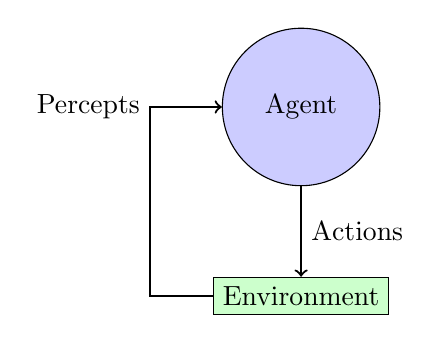
\begin{tikzpicture}[scale=0.8]
\node[circle, draw, fill=blue!20, minimum width=2cm] (agent) at (0,0) {Agent};
\node[rectangle, draw, fill=green!20] (env) at (0,-3) {Environment};
\draw[->, thick] (agent) -- node[right] {Actions} (env);
\draw[->, thick] (env.west) -- ++(-1,0) |- node[left] {Percepts} (agent.west);
\end{tikzpicture}
\end{columns}
\end{frame}

% Evolution from Single to Multi-Agent
\begin{frame}{Evolution: From Single Agent to Multi-Agent Systems}
\begin{center}
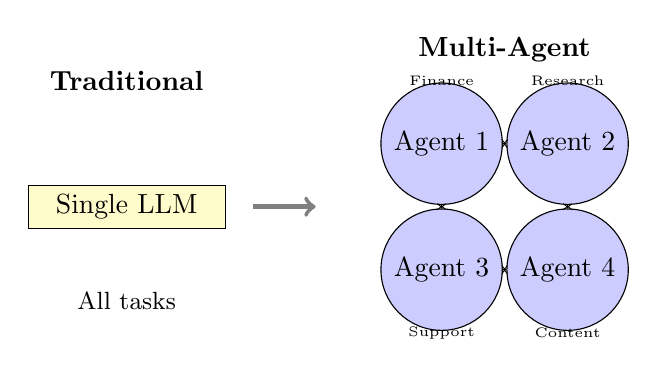
\begin{tikzpicture}[scale=0.8]
% Single Agent
\node[rectangle, draw, fill=yellow!20, minimum width=2.5cm] (single) at (-4,0) {Single LLM};
\node (task1) at (-4,-1.5) {\small All tasks};

% Arrow
\draw[->, ultra thick, gray] (-2,0) -- (-1,0);

% Multi-Agent
\node[circle, draw, fill=blue!20] (agent1) at (1,1) {Agent 1};
\node[circle, draw, fill=blue!20] (agent2) at (3,1) {Agent 2};
\node[circle, draw, fill=blue!20] (agent3) at (1,-1) {Agent 3};
\node[circle, draw, fill=blue!20] (agent4) at (3,-1) {Agent 4};

\node (spec1) at (1,2) {\tiny Finance};
\node (spec2) at (3,2) {\tiny Research};
\node (spec3) at (1,-2) {\tiny Support};
\node (spec4) at (3,-2) {\tiny Content};

\draw[<->, dashed] (agent1) -- (agent2);
\draw[<->, dashed] (agent1) -- (agent3);
\draw[<->, dashed] (agent2) -- (agent4);
\draw[<->, dashed] (agent3) -- (agent4);

% Labels
\node at (-4,2) {\textbf{Traditional}};
\node at (2,2.5) {\textbf{Multi-Agent}};
\end{tikzpicture}
\end{center}

\vspace{0.3cm}

\begin{columns}
\column{0.5\textwidth}
\textbf{Single Agent Limitations:}
\begin{itemize}
    \item Jack of all trades, master of none
    \item Single point of failure
    \item Context length limitations
    \item No parallel processing
\end{itemize}

\column{0.5\textwidth}
\textbf{Multi-Agent Advantages:}
\begin{itemize}
    \item Specialized expertise
    \item Parallel task execution
    \item Fault tolerance
    \item Scalability
\end{itemize}
\end{columns}
\end{frame}

% Multi-Agent Systems Theory
\begin{frame}{Multi-Agent Systems (MAS) - Core Concepts}
\begin{columns}
\column{0.5\textwidth}
\textbf{Definition:}
\begin{quote}
A Multi-Agent System consists of multiple intelligent agents that interact to solve problems beyond the capabilities of individual agents.
\end{quote}

\textbf{Key Properties:}
\begin{itemize}
    \item \textbf{Distribution} - No central control
    \item \textbf{Cooperation} - Agents work together
    \item \textbf{Coordination} - Organized actions
    \item \textbf{Negotiation} - Conflict resolution
\end{itemize}

\column{0.5\textwidth}
\textbf{Communication Patterns:}
\begin{itemize}
    \item \faIcon{arrow-right} \textbf{Pipeline} - Sequential processing
    \item \faIcon{project-diagram} \textbf{Graph} - Complex workflows
    \item \faIcon{users} \textbf{Collaborative} - Team-based
    \item \faIcon{comments} \textbf{Conversational} - Dialogue-based
\end{itemize}

\vspace{0.3cm}
\textbf{Coordination Strategies:}
\begin{itemize}
    \item Centralized orchestration
    \item Peer-to-peer communication
    \item Blackboard systems
    \item Market-based coordination
\end{itemize}
\end{columns}
\end{frame}

% Why Build Multi-Agent Systems?
\begin{frame}{Why Build Multi-Agent Systems?}

\begin{columns}
\column{0.33\textwidth}
\textbf{1. Specialization}
\begin{itemize}
    \item Domain expertise
    \item Optimized prompts
    \item Specific tools
    \item Targeted training
\end{itemize}

\column{0.33\textwidth}
\textbf{2. Reliability}
\begin{itemize}
    \item Fault isolation
    \item Error recovery
    \item Load balancing
    \item Redundancy
\end{itemize}

\column{0.33\textwidth}
\textbf{3. Scalability}
\begin{itemize}
    \item Add agents easily
    \item Parallel processing
    \item Resource optimization
    \item Modular growth
\end{itemize}
\end{columns}

\vspace{0.5cm}

\begin{center}
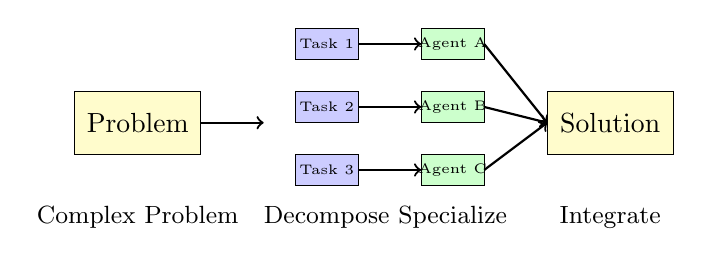
\begin{tikzpicture}[scale=0.8]
\draw[fill=yellow!20] (0,0) rectangle (2,1) node[pos=.5] {Problem};
\draw[->, thick] (2,0.5) -- (3,0.5);

% Decomposition
\draw[fill=blue!20] (3.5,1.5) rectangle (4.5,2) node[pos=.5, font=\tiny] {Task 1};
\draw[fill=blue!20] (3.5,0.5) rectangle (4.5,1) node[pos=.5, font=\tiny] {Task 2};
\draw[fill=blue!20] (3.5,-0.5) rectangle (4.5,0) node[pos=.5, font=\tiny] {Task 3};

% Agents
\draw[fill=green!20] (5.5,1.5) rectangle (6.5,2) node[pos=.5, font=\tiny] {Agent A};
\draw[fill=green!20] (5.5,0.5) rectangle (6.5,1) node[pos=.5, font=\tiny] {Agent B};
\draw[fill=green!20] (5.5,-0.5) rectangle (6.5,0) node[pos=.5, font=\tiny] {Agent C};

% Arrows
\draw[->, thick] (4.5,1.75) -- (5.5,1.75);
\draw[->, thick] (4.5,0.75) -- (5.5,0.75);
\draw[->, thick] (4.5,-0.25) -- (5.5,-0.25);

% Solution
\draw[->, thick] (6.5,1.75) -- (7.5,0.5);
\draw[->, thick] (6.5,0.75) -- (7.5,0.5);
\draw[->, thick] (6.5,-0.25) -- (7.5,0.5);
\draw[fill=yellow!20] (7.5,0) rectangle (9.5,1) node[pos=.5] {Solution};

\node at (1,-1) {\small Complex Problem};
\node at (4,-1) {\small Decompose};
\node at (6,-1) {\small Specialize};
\node at (8.5,-1) {\small Integrate};
\end{tikzpicture}
\end{center}
\end{frame}

% Framework Paradigms
\begin{frame}{Agent Framework Paradigms}

\begin{columns}
\column{0.5\textwidth}
\textbf{1. Workflow-Based (LangGraph)}
\begin{itemize}
    \item State machines
    \item Directed graphs
    \item Conditional routing
    \item Example: Financial analysis pipeline
\end{itemize}

\vspace{0.3cm}

\textbf{2. Role-Based (CrewAI)}
\begin{itemize}
    \item Team metaphor
    \item Defined roles \& goals
    \item Task delegation
    \item Example: Research team
\end{itemize}

\column{0.5\textwidth}
\textbf{3. Conversational (AutoGen)}
\begin{itemize}
    \item Natural dialogue
    \item Group discussions
    \item Turn-taking protocols
    \item Example: Brainstorming session
\end{itemize}

\vspace{0.3cm}

\textbf{4. Assistant-Based (Phidata)}
\begin{itemize}
    \item Single purpose agents
    \item Tool integration
    \item Memory management
    \item Example: Customer service bot
\end{itemize}
\end{columns}

\vspace{0.3cm}
\begin{center}
\colorbox{yellow!20}{\textbf{Key Insight:} Different problems require different coordination patterns}
\end{center}
\end{frame}

% Challenges in Multi-Agent Systems
\begin{frame}{Challenges in Multi-Agent Systems}

\begin{columns}
\column{0.5\textwidth}
\textbf{Technical Challenges:}
\begin{itemize}
    \item \faIcon{exchange-alt} \textbf{Communication}
    \begin{itemize}
        \item Message passing protocols
        \item State synchronization
        \item Data serialization
    \end{itemize}
    
    \item \faIcon{sync} \textbf{Coordination}
    \begin{itemize}
        \item Task scheduling
        \item Conflict resolution
        \item Deadlock prevention
    \end{itemize}
    
    \item \faIcon{eye} \textbf{Observability}
    \begin{itemize}
        \item Distributed tracing
        \item Performance monitoring
        \item Debug complexity
    \end{itemize}
\end{itemize}

\column{0.5\textwidth}
\textbf{Practical Challenges:}
\begin{itemize}
    \item \faIcon{dollar-sign} \textbf{Cost Management}
    \begin{itemize}
        \item Multiple API calls
        \item Resource allocation
        \item Provider selection
    \end{itemize}
    
    \item \faIcon{tachometer-alt} \textbf{Performance}
    \begin{itemize}
        \item Latency accumulation
        \item Bottleneck identification
        \item Scaling issues
    \end{itemize}
    
    \item \faIcon{shield-alt} \textbf{Reliability}
    \begin{itemize}
        \item Error propagation
        \item Failure recovery
        \item Quality assurance
    \end{itemize}
\end{itemize}
\end{columns}

\vspace{0.3cm}
\begin{center}
\textbf{Our Solution:} Framework-agnostic architecture with unified observability
\end{center}
\end{frame}

% === TRANSITION TO IMPLEMENTATION ===

% Transition Slide
\begin{frame}{From Theory to Practice}
\begin{center}
\Large
\textbf{How We Applied These Concepts}\\
\vspace{0.5cm}
\normalsize
Building a real-world multi-agent system with:\\
\vspace{0.3cm}
\begin{itemize}
    \item 16 specialized agents
    \item 4 different frameworks
    \item 5 domain categories
    \item Production-ready deployment
\end{itemize}

\vspace{0.5cm}
\textbf{Let's see how theory becomes practice...}
\end{center}
\end{frame}

% === IMPLEMENTATION SECTION (Original slides continue) ===

% System Overview
\begin{frame}{Our Implementation: System Overview}
\begin{columns}
\column{0.5\textwidth}
\textbf{What We Built:}
\begin{itemize}
    \item 16 specialized AI agents
    \item 5 domain categories
    \item 4 different frameworks
    \item Docker-based deployment
    \item Unified dashboard
\end{itemize}

\column{0.5\textwidth}
\textbf{Key Numbers:}
\begin{itemize}
    \item \faIcon{robot} 16 Agents
    \item \faIcon{code-branch} 4 Frameworks
    \item \faIcon{eye} 3 Observability Platforms
    \item \faIcon{cloud} 10+ AI Providers
    \item \faIcon{docker} 8+ Docker Services
\end{itemize}
\end{columns}

\vspace{0.3cm}
\begin{center}
\colorbox{green!20}{Applying MAS theory to solve real business problems}
\end{center}
\end{frame}

% Architecture Overview
\begin{frame}{System Architecture}
\begin{center}
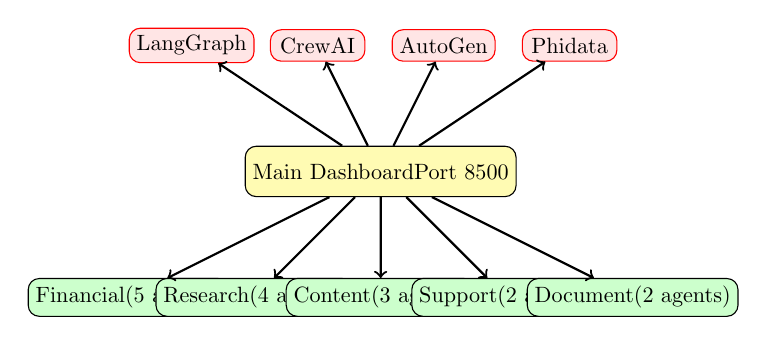
\begin{tikzpicture}[scale=0.8, transform shape,
  box/.style={rectangle, rounded corners, minimum width=2cm, minimum height=0.8cm, text centered, draw=black, fill=blue!20},
  agent/.style={rectangle, rounded corners, minimum width=1.8cm, minimum height=0.6cm, text centered, draw=black, fill=green!20},
  framework/.style={rectangle, rounded corners, minimum width=1.5cm, minimum height=0.5cm, text centered, draw=red, fill=red!10}
]

% Main Dashboard
\node[box, fill=yellow!30] (dashboard) at (0,0) {Main Dashboard\\Port 8500};

% Frameworks
\node[framework] (langgraph) at (-3,2) {LangGraph};
\node[framework] (crewai) at (-1,2) {CrewAI};
\node[framework] (autogen) at (1,2) {AutoGen};
\node[framework] (phidata) at (3,2) {Phidata};

% Agent Categories
\node[agent] (financial) at (-4,-2) {Financial\\(5 agents)};
\node[agent] (research) at (-2,-2) {Research\\(4 agents)};
\node[agent] (content) at (0,-2) {Content\\(3 agents)};
\node[agent] (support) at (2,-2) {Support\\(2 agents)};
\node[agent] (document) at (4,-2) {Document\\(2 agents)};

% Connections
\draw[->, thick] (dashboard) -- (langgraph);
\draw[->, thick] (dashboard) -- (crewai);
\draw[->, thick] (dashboard) -- (autogen);
\draw[->, thick] (dashboard) -- (phidata);

\draw[->, thick] (dashboard) -- (financial);
\draw[->, thick] (dashboard) -- (research);
\draw[->, thick] (dashboard) -- (content);
\draw[->, thick] (dashboard) -- (support);
\draw[->, thick] (dashboard) -- (document);

\end{tikzpicture}
\end{center}

\textbf{Design Principles Applied:}
\begin{itemize}
    \item \textbf{Specialization:} Each agent focuses on specific domain
    \item \textbf{Coordination:} Central dashboard orchestrates agents
    \item \textbf{Flexibility:} Multiple frameworks for different use cases
\end{itemize}
\end{frame}

% Framework Selection in Practice
\begin{frame}{Framework Selection in Practice}
\begin{table}
\centering
\small
\begin{tabular}{llll}
\toprule
\textbf{Framework} & \textbf{Paradigm} & \textbf{Best For} & \textbf{Our Usage} \\
\midrule
LangGraph & Workflow & Complex pipelines & Financial Analysis \\
CrewAI & Role-based & Team collaboration & Stock Analysis \\
AutoGen & Conversational & Discussions & Research Agent \\
Phidata & Assistant & Simple tasks & Basic Agents \\
\bottomrule
\end{tabular}
\end{table}

\vspace{0.5cm}

\textbf{Real Examples from Our System:}
\begin{itemize}
    \item \textbf{LangGraph:} Financial analysis with 7 sub-agents using conditional routing
    \item \textbf{CrewAI:} Stock analysis team with technical \& fundamental analysts
    \item \textbf{AutoGen:} Research conversations with iterative refinement
    \item \textbf{Phidata:} Simple Q\&A assistants with memory
\end{itemize}
\end{frame}

% Agent Portfolio - Financial
\begin{frame}{Agent Portfolio - Applying Specialization}
\begin{columns}
\column{0.6\textwidth}
\textbf{Financial Domain (5 agents)}
\begin{itemize}
    \item Multi-Agent Financial Analysis
    \item Stock Analysis Extended
    \item Finance Advisor
    \item Stock Analysis
    \item Competitive Intel
\end{itemize}

\textbf{Research Domain (4 agents)}
\begin{itemize}
    \item ARIA (AutoGen Research)
    \item MARIA (Medical Research)
    \item Research V2
    \item Insights Explorer
\end{itemize}

\column{0.4\textwidth}
\textbf{Content \& Support}
\begin{itemize}
    \item AI Content Creation
    \item Customer Support
    \item Support Triage
    \item Resume Screening
\end{itemize}

\textbf{Document Processing}
\begin{itemize}
    \item Legal Review
    \item Handwriting Analysis
\end{itemize}
\end{columns}

\vspace{0.3cm}
\begin{center}
\colorbox{blue!20}{Each agent specialized for its domain = Better performance}
\end{center}
\end{frame}

% Solving MAS Challenges
\begin{frame}{How We Solved MAS Challenges}

\begin{columns}
\column{0.5\textwidth}
\textbf{Challenge $\rightarrow$ Solution}

\faIcon{exchange-alt} \textbf{Communication}
\begin{itemize}
    \item Unified agent interface
    \item Standard message format
    \item REST API endpoints
\end{itemize}

\faIcon{eye} \textbf{Observability}
\begin{itemize}
    \item 3-platform integration
    \item Distributed tracing
    \item Unified logging
\end{itemize}

\column{0.5\textwidth}
\faIcon{dollar-sign} \textbf{Cost Management}
\begin{itemize}
    \item Multi-provider support
    \item Automatic fallback
    \item Free tier options (HuggingFace)
\end{itemize}

\faIcon{rocket} \textbf{Deployment}
\begin{itemize}
    \item Docker containerization
    \item Service orchestration
    \item Health monitoring
\end{itemize}
\end{columns}

\vspace{0.3cm}
\begin{center}
\textbf{Result:} Production-ready multi-agent system
\end{center}
\end{frame}

% Key Features
\begin{frame}{Key Features - Theory in Action}
\begin{columns}
\column{0.5\textwidth}
\textbf{\faIcon{plug} Multi-Provider Support}
\begin{itemize}
    \item OpenAI GPT-4
    \item Anthropic Claude
    \item Google Gemini
    \item HuggingFace Models
    \item Automatic fallback
\end{itemize}

\textit{Solves: Cost \& reliability challenges}

\column{0.5\textwidth}
\textbf{\faIcon{chart-line} Observability}
\begin{itemize}
    \item LangSmith tracing
    \item AgentOps monitoring
    \item Langfuse analytics
    \item Unified logging
    \item Performance tracking
\end{itemize}

\textit{Solves: Debugging \& monitoring challenges}
\end{columns}

\vspace{0.5cm}

\textbf{\faIcon{docker} Production Deployment}
\begin{itemize}
    \item Containerized microservices (isolation)
    \item Docker Compose orchestration (coordination)
    \item Service discovery (communication)
    \item Health monitoring (reliability)
\end{itemize}
\end{frame}

% Demo Preparation
\begin{frame}{Demo Overview}
\textbf{What We'll Demonstrate:}

\begin{enumerate}
    \item \textbf{Main Dashboard} - Central coordination in action
    \begin{itemize}
        \item Agent status monitoring
        \item Service health checks
    \end{itemize}
    
    \item \textbf{Workflow-Based Agent} (LangGraph)
    \begin{itemize}
        \item Financial analysis with conditional routing
        \item Multi-agent collaboration
    \end{itemize}
    
    \item \textbf{Role-Based Agent} (CrewAI)
    \begin{itemize}
        \item Stock analysis team
        \item Task delegation
    \end{itemize}
    
    \item \textbf{Conversational Agent} (AutoGen)
    \begin{itemize}
        \item Research discussions
        \item Iterative refinement
    \end{itemize}
\end{enumerate}

\vspace{0.3cm}
\begin{center}
\textbf{See theory become practice!}
\end{center}
\end{frame}

% Access Information
\begin{frame}{System Access}
\begin{center}
\Large
\textbf{Main Dashboard}\\
\vspace{0.3cm}
\faIcon{globe} \texttt{http://localhost:8500}\\
\vspace{1cm}

\normalsize
\begin{tabular}{ll}
\toprule
\textbf{Service} & \textbf{Port} \\
\midrule
Main Dashboard & 8500 \\
Legal Document Review & 8501 \\
Customer Support & 8502 \\
Finance Advisor & 8503 \\
Stock Analysis Extended & 8507 \\
Support Triage & 8506 \\
\bottomrule
\end{tabular}
\end{center}

\vspace{0.5cm}
\textbf{Note:} Ensure Docker services are running via \texttt{docker-compose up}
\end{frame}

% Key Takeaways
\begin{frame}{Key Takeaways}

\textbf{Theoretical Insights:}
\begin{itemize}
    \item Multi-agent systems enable specialization and scalability
    \item Different coordination paradigms suit different problems
    \item Communication and observability are critical challenges
\end{itemize}

\vspace{0.3cm}

\textbf{Practical Achievements:}
\begin{itemize}
    \item Successfully integrated 4 different frameworks
    \item Deployed 16 specialized agents in production
    \item Solved real-world business problems
    \item Created reusable patterns for MAS development
\end{itemize}

\vspace{0.5cm}
\begin{center}
\Large
\textbf{Questions before we start the demo?}
\end{center}
\end{frame}

% Thank You / Demo Time
\begin{frame}
\begin{center}
\Huge
\textbf{Live Demo}\\
\vspace{1cm}
\Large
Let's see the multi-agent system in action!\\
\vspace{0.5cm}
\normalsize
Starting with the Main Dashboard\\
\texttt{http://localhost:8500}
\end{center}
\end{frame}

\end{document}